%! Author = boldi
%! Date = 08/06/2026

% Preamble
\documentclass[11pt]{article}

% Packages
\usepackage{bookmark}
\usepackage{xcolor}
\hypersetup{colorlinks}
\usepackage{csquotes}
\usepackage{multirow}
\usepackage{booktabs}
\usepackage{makecell}
\usepackage{svg}

\usepackage{amsmath}
\usepackage{stmaryrd}
\SetSymbolFont{stmry}{bold}{U}{stmry}{m}{n}

\usepackage{amsthm,thmtools}
\theoremstyle{definition}
\newtheorem{theorem}{Theorem}
\newtheorem{lemma}[theorem]{Lemma}
\newtheorem{proposition}[theorem]{Proposition}
\newtheorem{definition}{Definition}

\usepackage{cleveref}

\usepackage[a4paper, total={6in, 8in}]{geometry}

\usepackage{macros/tikzfig}
\input{macros/floquet.tikzstyles}
\input{macros/floquet.tikzdefs}

\newcommand{\code}[1]{\left\llbracket#1\right\rrbracket}

\setcounter{MaxMatrixCols}{20}

\title{CSSCat: scalable fault-tolerant CSS-state preparation}
%\title{CSSCat: fault-tolerant CSS-states by construction}
\author{}

% Document
\begin{document}

\maketitle

\section{Theoretical Framework}\label{sec:the-theory}

\subsection{ZX-Calculus Representation of CSS Codes}
Any Calderbank-Shor-Steane (CSS) quantum error-correcting code can be natively represented as a ZX-diagram~\cite{kissingerPhasefreeZXDiagrams2022}.
This representation is constructed by mapping the generators of the stabilizer group and the logical operators of the code into a network of interconnected spiders.

\begin{proposition}
  Given a set of stabilizers of any CSS-QECC\@.
  We can represent a ZX-diagram fault-tolerantly preparing this state.
\end{proposition}

We will use the $\code{7,1,3}$ Steane as a running example, whose stabilizer generators can be explicitly written as:
\begin{gather}
Z_{1} Z_{2} Z_{3} Z_{4} \quad
Z_{2} Z_{3} Z_{5} Z_{6} \quad
Z_{3} Z_{4} Z_{6} Z_{7} \quad
X_{1} X_{2} X_{3} X_{4} \quad
X_{2} X_{3} X_{5} X_{6} \quad
X_{3} X_{4} X_{6} X_{7}
\end{gather}

From these stabilizers, one can construct encoders for the code or the fault-tolerant state preparation ZX-diagrams.

\begin{equation}
  \ket{\overline{0}}\ = \ \tikzfig{figures/steane-zero}
  \qquad
  \qquad
  \ket{\overline{+}}\ = \ \tikzfig{figures/steane-plus}
  \label{eq:logical-basis-states}
\end{equation}
In this representation, the connectivity of the X and Z spiders denote the stabilizers of the code.
Note that we are marking internal edges with purple color, denoting that these are \enquote{perfect} edges.
As established in Section \ref{sec:preliminaries}, a perfect edge serves as a mathematical specification of an idealized, noiseless logical correlation.
Because physical hardware cannot natively execute noiseless operations, these edges serve only as an intermediate representation.
They must be eliminated from the diagram to extract a valid, physically realizable fault-tolerant quantim circuit.

\subsection{Fault-Equivalent Edge Elimination}

To extract a physically realizable quantum circuit, we must find a fault-equivalent ZX-diagram with no idealized edges.
To achieve this, we introduce the following fault-equivalent (FE) ZX-rewrite rule:
\begin{proposition}
  \label{prop:unidealize}
  An idealized edge can be unidealized under CSS-noise if the edge is between a Z- and an X-spider, and both spiders have at least 1 unidealized leg:
  \begin{equation}
    \tikzfig{figures/johns-rule}
  \end{equation}
\end{proposition}
\begin{proof}
  \textbf{TODO}
\end{proof}

%\begin{equation}
%  \tikzfig{figures/steane-plus-unidealize}
%\end{equation}

\subsection{Bipartite Structural Constrains}

If we wanted to apply this rewrite rule to unidealize all internal edges, we would fail because internal spiders have no unidealized legs.
For this rewrite to enable the removal of all idealized edges, we need our ZX-diagram to represent a bipartite graph state.
\begin{proposition}
  Given a ZX-diagram representing a bipartite graph state with idealized internal edges.
  We can unidealize all internal edges.
\end{proposition}
While this might seem like a very particular property, it turns out that any CSS state can be represented in this form:
\begin{proposition}
  Every CSS state can be represented as a bipartite graph state.
\end{proposition}

For our running example, we can find a bipartite ZX-diagram where all nodes are boundary, and then unrealize all internal edges as follows:
\begin{equation}
  \tikzfig{figures/steane-zero-basis-change}
  \label{eq:bipartite-state}
\end{equation}

\subsection{Spider Decompositions and Measurement-Free Connectivity}
Once the bipartite ZX-diagram is free of perfect edges, the remaining graph consists of physical, but high-degree spiders, which cannot natively be realized using 2-qubit gates.
In order to obtain a ZX-diagram from which a circuit can be extracted, each high-degree spider must be fault-equivalently decomposed into a network of degree-3 spiders.
This can be done using SpiderCat~\cite{spidercat}.

For example:
\begin{equation}
  \tikzfig{figures/steane-zero-unfused}
\end{equation}
This final ZX-diagram fault-tolerantly prepares the $\ket{\overline 0}$ state for the Steane code.

\section{Circuit Extraction}

Once a ZX-diagram is obtained, the only thing that remains is extracting a quantum circuit.
However, this, in general, is computationally hard as the problem is closely related to finding a path-cover with $n$ paths on the ZX-diagram with additional constraints.
While for smaller codes this is feasible, for larger codes, solving this problem will likely become untraceable.

In order to tractably solve this problem, we want to utilize spanning trees on individual 3-regular ZX-diagrams, which serve as blueprints for circuit extraction for the CAT sates.
Then, we will only need to combine these spanning trees so that global blueprint can be obtained.

A naive approach to obtaining a quantum circuit would be to directly utilize the CAT states and implement the connections between them as Bell-state measurements:
\begin{equation}
  \tikzfig{figures/steane-zero-naive-se}
\end{equation}
However, this approach requires a very large number of ancilla qubits, and it does not utilize the fact that legs between a Z- and an X-spider can often be extracted as CNOT gates.
In fact, each internal edge in the original diagram is extracted as 3 CNOT gates and 2 measurements:
one CNOT gate for each output of the two CAT states, and an additional CNOT for the Bell measurement that also needs two measurements.

To reduce the resource requirements, we introduce two fault equivalent rewrites, both of which can eliminate a CNOT gate and a measurement per application.
\begin{proposition}[Direct CNOT condition]
  Given a CAT state with an output qubit $q$ which is prepared using only a state preparation and a CNOT gate $a \to q$ gate.
  Let $q$ be followed by another CNOT gate $q \to b$ and a measurement in the conjugate basis.
  This circuit is fault-equivalent to a circuit where all operations on $q$ are replaced with a singed CNOT gate $a \to b$.
  \label{prop:cat-reduction-1}
  \begin{equation*}\label{eq:cat-part-1}
    \tikzfig{figures/cat-part-1}
  \end{equation*}
\end{proposition}

\begin{proposition}[Flag-delegation condition]
  Given a CAT state with an output qubit $q$ on which the last CNOT gate involves a flag qubit $f$.
  Furthermore, if $a \to f$ and $q \to f$ are the two CNOT gates applied to $f$, then $q \to f$ must happen before $a \to f$.
  Let $q$ be followed by another CNOT gate $q \to b$ and a measurement in the conjugate basis.
  This circuit is fault-equivalent to a circuit where qubit $f$ is removed and is replaced with CNOTs $q \to b$, $a \to q$, followed by the flag measurement applied to $q$.
  \label{prop:cat-reduction-2}
  \begin{equation*}\label{eq:cat-part-2}
    \tikzfig{figures/cat-part-2-fe}
  \end{equation*}
\end{proposition}

\begin{proposition}
  Given a fault-tolerant CAT state prepared using state preparations, CNOT gates, and measurements.
  On any of its output qubits, the last operations is a CNOT gate, and this CNOT gate is either:
  \begin{enumerate}
    \item the only CNOT gate applied to the qubit, or,
    \item a CNOT between a flag and the qubit.
  \end{enumerate}
\end{proposition}
\begin{proof}
  The only thing that this eliminates is for a CNOT gate to be last if it was applied between two non-flag qubits.
  [TODO: cannot happen because then the circuit is not FT...]
\end{proof}

\begin{proposition}\label{prop:connection_overhead}
  Consider a CAT state decomposed into a physical circuit.
  If all but one of its boundary legs satisfy either the direct CNOT condition or the flag-delegation condition, then the entire spider can be directly connected to the broader CSS state without requiring intermediate Bell-state measurements.
  The leg not satisfying either of these conditions serves as the output of the spider.
\end{proposition}

While standard SpiderCat minimizes gate counts, it does not guarantee that extracted circuits satisfy \cref{prop:connection_overhead}.
In particular, SpiderCat does not have conditions to satisfy the flag-delegation condition because the ordering of the CNOTs applied to the flag qubit can be arbitrary.

\subsection{Constructing appropriate CAT states}

We implement a modified version of SpiderCat that enables the application of \cref{prop:connection_overhead} for each spider.
For this to be the case, all we need to ensure is that for all but one output qubits, whenever the last CNOT is between a flag and the qubit, this CNOT must be the first CNOT applied to the flag.

To enable the extraction of such CAT states, we extend the SpiderCat pipeline with a DAG that dictates the order in which nodes are traversed during circuit extraction.
In particular, the order in which we process nodes during circuit extraction is dictated by the topological generations of the DAG\@.
Then, we can artificially insert directed edges that correspond to the constraint that the if the final CNOT gate on a qubit is applied to a flag, it should be the first CNOT of the flag.
This artificial directed graph will not be a DAG, because the newly inserted edges can easily form a causal cycle.
However, this can be salvaged by removing a flag CNOT constraint from the directed graph if it then forms a DAG\@.
The edges from which the constraint is removed will serve es the output of the spider.

\begin{figure}
  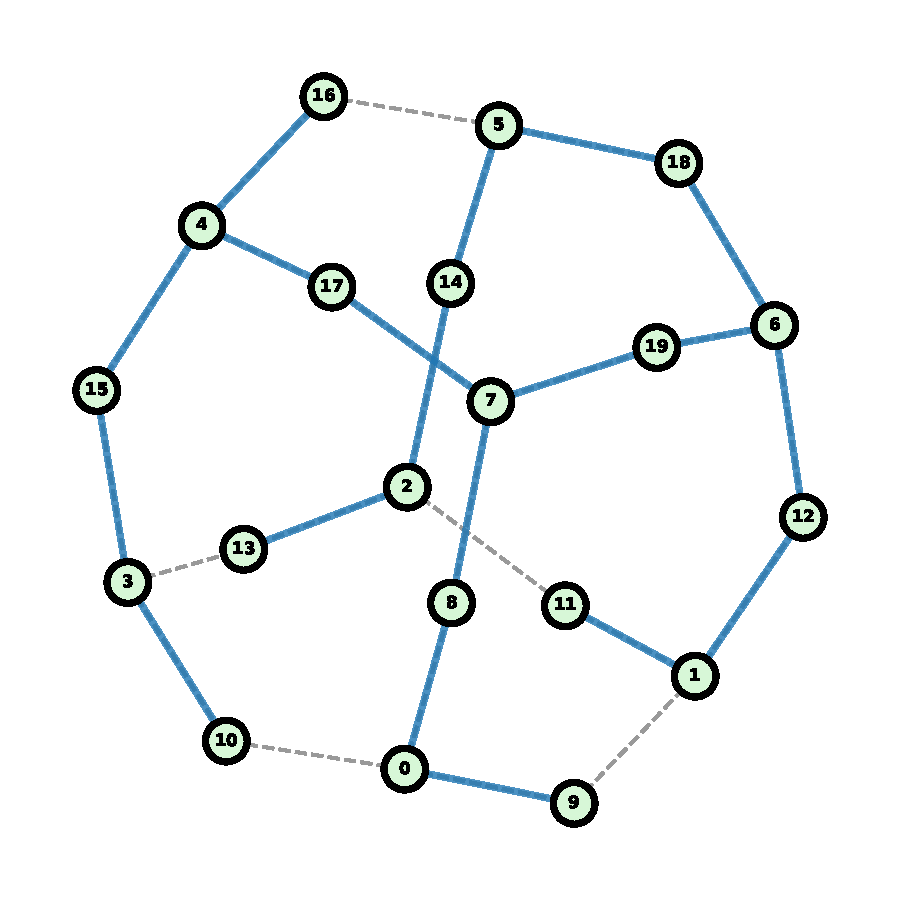
\includegraphics[width=0.32\textwidth]{figures/cat_state_base}
  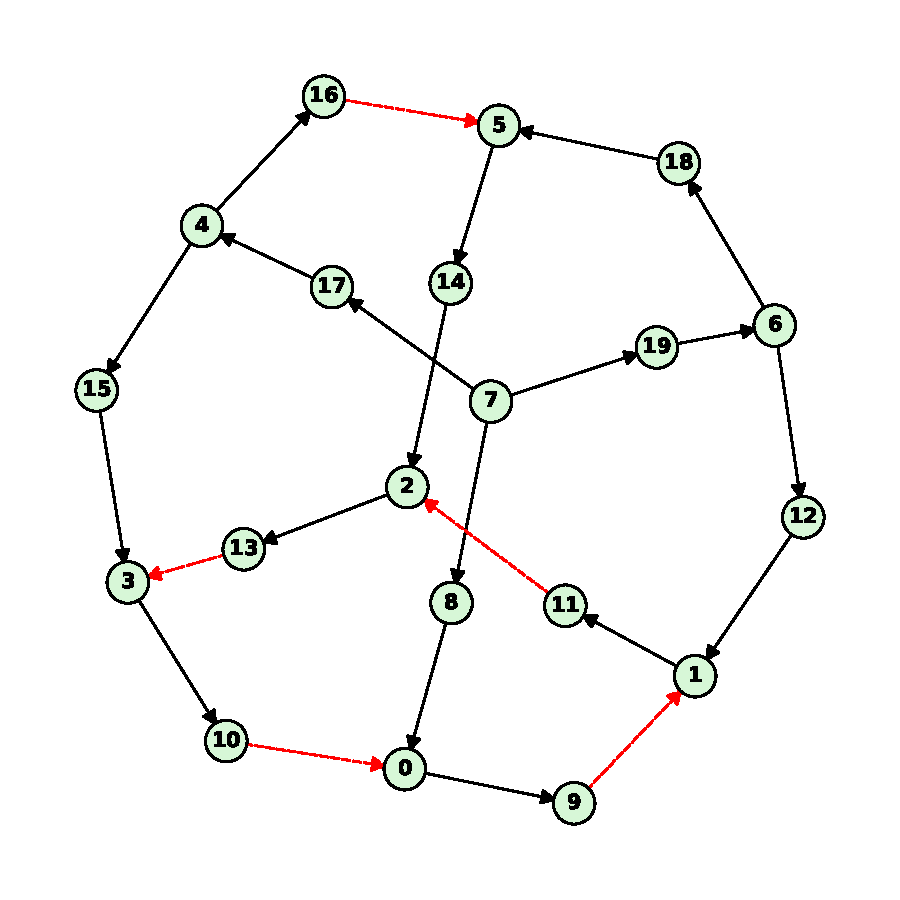
\includegraphics[width=0.32\textwidth]{figures/digraph_base}
  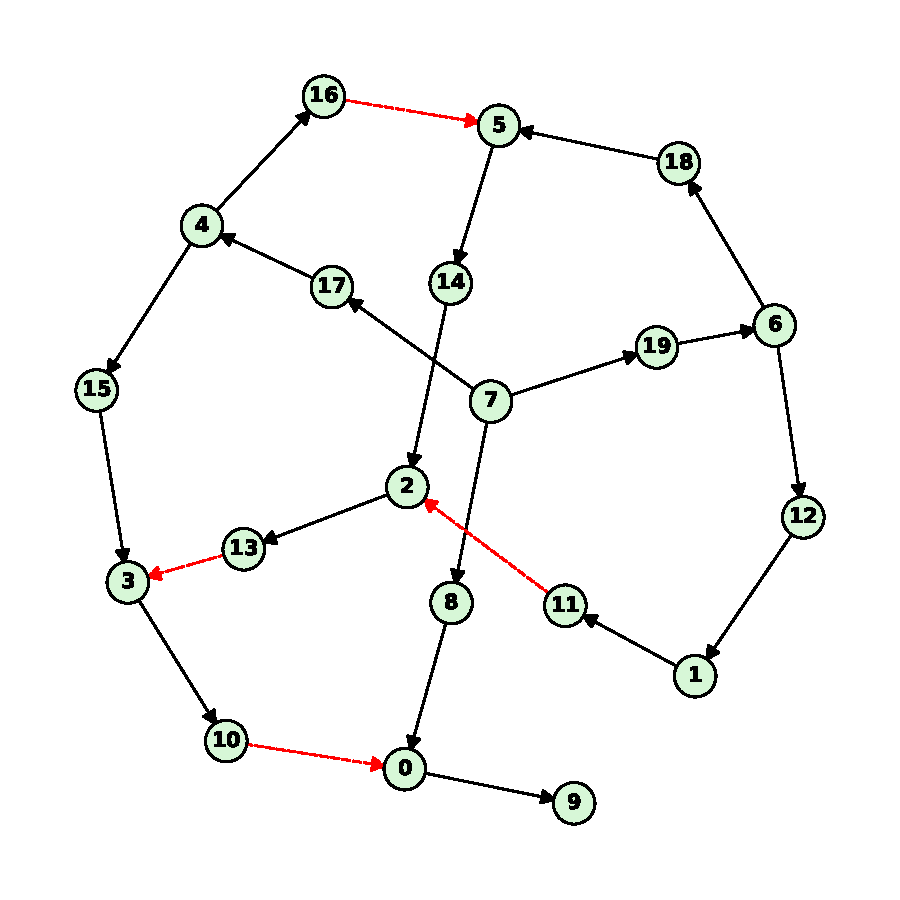
\includegraphics[width=0.32\textwidth]{figures/resolved_DAG}

  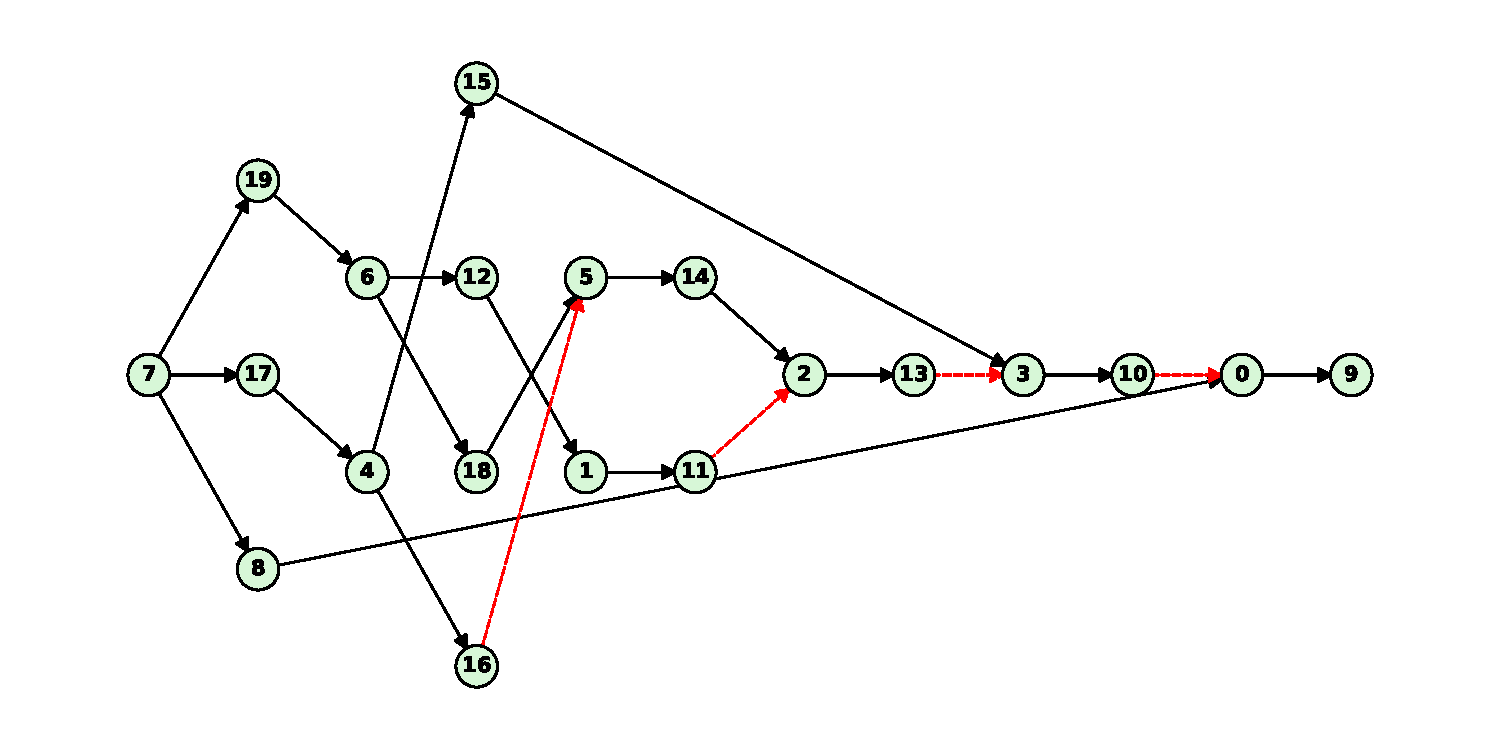
\includegraphics[width=0.5\textwidth]{figures/resolved_DAG_generational}
  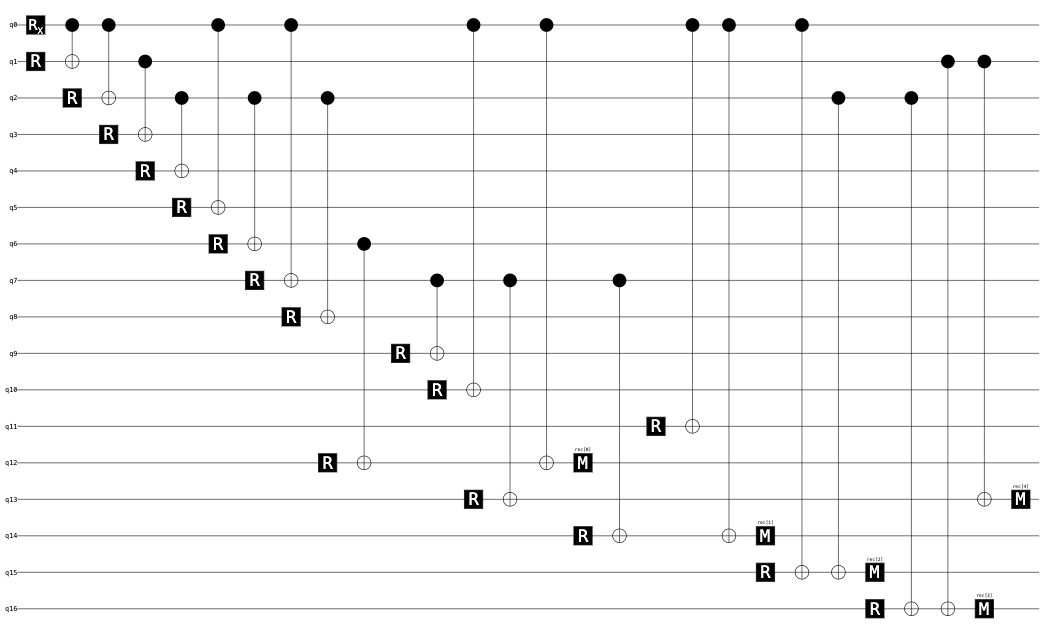
\includegraphics[width=0.5\textwidth]{figures/well_ordered_cat_state.png}
%  \includesvg[]{figures/well_ordered_cat_state.svg}
\end{figure}


\section{Simulation Results}

\begin{table*}[h]
\centering
\scriptsize
\begin{tabular}{l c c c c c c c c}
\toprule
\makecell[l]{QEC Code \\ \& State} & \makecell{CX \\ Count} & \makecell{Flag \\ Count} & \makecell{Reuse \\ Strategy} & \makecell{Sim.\@ \\ Qubits} & Depth & \makecell{Exp.\@ Circ.\@ \\ Volume} & \makecell{Log.\@ Error \\ Rate} & \makecell{Acc.\@ \\ Rate} \\
\midrule
\multirow{2}{*}{\makecell[l]{$\code{7, 1, 3}$ Steane $\ket{\overline{0}}$}} & \multirow{2}{*}{17} & \multirow{2}{*}{4} & Naive & 11 & 5 & 55 & $2.40\! \times\! 10^{-5}$ & 98.31\% \\
 &  &  & Aggressive & 10 & 8 & 81 & $2.49\! \times\! 10^{-5}$ & 98.33\% \\
\midrule
\multirow{2}{*}{\makecell[l]{$\code{9, 1, 3}$ rot.\@ surface $\ket{\overline{0}}$}} & \multirow{2}{*}{12} & \multirow{2}{*}{2} & Naive & 11 & 5 & 55 & $1.63\! \times\! 10^{-5}$ & 99.13\% \\
 &  &  & Aggressive & 10 & 8 & 80 & $1.68\! \times\! 10^{-5}$ & 99.13\% \\
\midrule
\multirow{2}{*}{\makecell[l]{$\code{17, 1, 5}$ color code $\ket{\overline{0}}$}} & \multirow{2}{*}{74} & \multirow{2}{*}{21} & Naive & 35 & 13 & 499 & $9.22\! \times\! 10^{-7}$ & 91.03\% \\
 &  &  & Aggressive & 27 & 35 & 1034 & $8.72\! \times\! 10^{-7}$ & 91.31\% \\
\midrule
\multirow{2}{*}{\makecell[l]{$\code{25, 1, 5}$ rot.\@ surface $\ket{\overline{0}}$}} & \multirow{2}{*}{78} & \multirow{2}{*}{21} & Naive & 44 & 11 & 533 & $6.47\! \times\! 10^{-7}$ & 90.75\% \\
 &  &  & Aggressive & 34 & 42 & 1566 & $7.98\! \times\! 10^{-7}$ & 91.14\% \\
\midrule
\multirow{2}{*}{\makecell[l]{$\code{20, 2, 6}$ self-dual $\ket{\overline{0}}$}} & \multirow{2}{*}{145} & \multirow{2}{*}{47} & Naive & 53 & 22 & 1443 & $3.10\! \times\! 10^{-8}$ & 80.77\% \\
 &  &  & Aggressive & 48 & 63 & 3738 & $5.93\! \times\! 10^{-8}$ & 80.88\% \\
\midrule
\multirow{2}{*}{\makecell[l]{$\code{23, 1, 7}$ Golay $\ket{\overline{0}}$}} & \multirow{2}{*}{241} & \multirow{2}{*}{82} & Naive & 83 & 22 & 2727 & $2.67\! \times\! 10^{-7}$ & 66.96\% \\
 &  &  & Aggressive & 64 & 106 & 10035 & $3.21\! \times\! 10^{-7}$ & 67.60\% \\
\midrule
\multirow{2}{*}{\makecell[l]{$\code{31, 1, 7}$ color code $\ket{\overline{0}}$}} & \multirow{2}{*}{211} & \multirow{2}{*}{69} & Naive & 79 & 23 & 2518 & $1.12\! \times\! 10^{-7}$ & 72.14\% \\
 &  &  & Aggressive & 63 & 90 & 7756 & $1.14\! \times\! 10^{-7}$ & 73.10\% \\
\midrule
\multirow{2}{*}{\makecell[l]{$\code{49, 1, 7}$ rot.\@ surface $\ket{\overline{0}}$}} & \multirow{2}{*}{228} & \multirow{2}{*}{70} & Naive & 87 & 23 & 2796 & $1.06\! \times\! 10^{-7}$ & 71.56\% \\
 &  &  & Aggressive & 80 & 81 & 9005 & $1.39\! \times\! 10^{-7}$ & 71.95\% \\
\midrule
\multirow{2}{*}{\makecell[l]{$\code{49, 1, 9}$ color code $\ket{\overline{0}}$}} & \multirow{2}{*}{402} & \multirow{2}{*}{133} & Naive & 133 & 30 & 8208 & $3.09\! \times\! 10^{-8}$ & 48.61\% \\
 &  &  & Aggressive & 113 & 149 & 33600 & $2.99\! \times\! 10^{-8}$ & 50.11\% \\
\midrule
\multirow{2}{*}{\makecell[l]{$\code{47, 1, 11}$ color code $\ket{\overline{0}}$}} & \multirow{2}{*}{955} & \multirow{2}{*}{349} & Naive & 233 & 53 & 116047 & $4.98\! \times\! 10^{-7}$ & 10.64\% \\
 &  &  & Aggressive & 201 & 419 & 737540 & $1.49\! \times\! 10^{-7}$ & 11.42\% \\
\midrule
\bottomrule
\end{tabular}
\caption{Simulation results across various QEC codes and qubit reuse strategies.}
\label{tab:sim_results}
\end{table*}


\iffalse
% ==========================================
% SECTION: THE PIPELINE
% ==========================================
\section{The Compilation Pipeline}\label{sec:the-pipeline}

To physicalize the theoretical constructs outlined in Section~\ref{sec:the-theory}, we introduce a comprehensive compilation pipeline. This algorithm accepts an arbitrary CSS code parity check matrix and deterministically outputs a highly optimized, fault-tolerant state preparation circuit. The pipeline operates in three distinct phases: (1) logical resource optimization to find the ideal bipartite basis, (2) topologically constrained spider generation to satisfy Proposition~\ref{prop:connection_overhead}, and (3) acyclic global edge routing to synthesize the final circuit.

\subsection{Phase 1: Resource Characterization and Basis Optimization}
Our pipeline begins by quantifying the logical resources required to prepare a given state.
Given an X or Z spider of degree $n$, we characterize the exact logical CNOT cost assuming a tolerance of $t$ faults.

The density lower bound, $\delta(t)$, governs the necessary graph density:
\begin{equation}
\delta(t) = \frac{\lceil(t+3)/2\rceil \lfloor(t+3)/2\rfloor}{\lceil(t+3)/2\rceil \lfloor(t+3)/2\rfloor + \lceil(t-3)/2\rceil \lfloor(t+3)/2\rfloor + \lfloor(t-3)/2\rfloor \lceil(t+3)/2\rceil}
\end{equation}

Because a degree-$n$ spider represents a cat state stabilized by a global parity operator, the maximum number of faults requiring correction is bounded: $t' = \min\left(t, \lfloor n/2 \rfloor - 1\right)$. By the handshaking lemma for 3-regular graphs, the final edge count $E$ and vertex count $V$ are determined by:
\begin{equation}
E = 3 \left\lceil \frac{\lceil n / \delta(t') \rceil}{3} \right\rceil, \quad V = \frac{2E}{3}
\end{equation}

The minimum number of flag qubits is $f(n, t) = \max\left(0, \lceil E - V + 2 \rceil - 1\right)$. The logical CNOT cost for a single isolated spider is bounded by: $C_{\text{spider}}(n, t) = n - 1 + 2f(n, t)$.

\subsubsection*{Row Optimization via Stochastic Basis Search}
For the state preparation method to be correct, the corresponding ZX diagram must represent a bipartite graph state (\cref{sec:the-theory}).
For any parity matrix $M$ in a systematic form, there is a corresponding bipartite ZX-diagram.
The total logical CNOT cost of the resulting circuit is:
\begin{equation}
C_{\text{total}}(M, t) = \sum_{\substack{c=1 \\ w_c > 1}}^c 2f(w_c + 1, t) + \sum_{r=1}^r \left[ w_r - 1 + 2f(w_r, t) \right]
\end{equation}
where $w_c$ and $w_r$ are the column and row Hamming weights.

Because finding the globally optimal basis over $\mathbb{F}_2$ can be computationally hard, Phase 1 employs a Monte Carlo optimization heuristic.
We randomly sample subsets of $r$ columns from $M$ to form $r \times r$ submatrices.
If a submatrix $M_{\text{sub}}$ is non-singular, we compute the row-equivalent matrix $M_{\text{new}} = (M_{\text{sub}}^{-1} M) \pmod 2$.
We evaluate $C_{\text{total}}(M_{\text{new}}, t)$ for each valid basis and retain the matrix that minimizes the total logical CNOT cost.

\subsection{Phase 2: Constrained Spider Decompositions via Simulated Annealing}
\textbf{[TODO: Draft Phase 2. Explain how the code translates individual spiders into physical structures.]}
\begin{itemize}
    \item Explain the necessity of the Minimum Diameter Spanning Forest (MDSF) to minimize circuit depth (longest root-to-leaf path).
    \item Explain the Simulated Annealing heuristic used to mutate the forest while preserving $k$-components.
    \item Detail the \textit{topological penalties} applied during generation (e.g., degree locking and penalizing leaf adjacency) that actively force the algorithm to satisfy Proposition \ref{prop:connection_overhead}.
    This is what transforms standard SpiderCat into your "Modified" version.
\end{itemize}

\subsubsection*{Dependency Graph Construction and Acyclic Resolution}

The dependency graph $D$ is constructed via a two-step topological mapping:
\begin{enumerate}
    \item \textbf{Tree Traversal Edges:} For every edge in the spanning forest $F$, we add a directed edge in $D$ originating from the root and flowing outward towards the leaves. This represents the sequential propagation of the cat state via CNOT gates.
    \item \textbf{Connection Scheduling Edges:} To guarantee the applicability of the flag-delegated rewrite (Eq.~\ref{eq:cat-part-2}), we must constrain the extraction order of the circuit. For every leaf node $l$ in $F$, we identify its neighbors in the original graph $G$ that are not connected via $F$. We append a directed edge from $l$ to each of these missing neighbors in $D$. By enforcing this dependency, the subsequent topological sort ensures that the final CNOT gate acting on a data qubit will deterministically be the initial CNOT gate of its corresponding flag.
\end{enumerate}

By enforcing these dependencies, the graph $D$ strictly models the causal requirements of our connection rewrites. However, because the underlying physical connectivity contains closed spatial loops, these temporal constraints inevitably introduce directed cycles into $D$. A directed cycle represents a temporal paradox in quantum circuit compilation: a sequence of operations must strictly precede itself, rendering extraction impossible.

To resolve this, we exploit the single degree of freedom permitted by Proposition~\ref{prop:connection_overhead}. The proposition dictates that exactly one boundary leg is exempt from the strict flag-delegated conditions, as it must serve as the dedicated logical output connecting the spider to the broader bipartite graph state.

Algorithmically, this translates to removing exactly one connection scheduling edge from $D$. Our modified SpiderCat implementation systematically iterates through all such edges, temporarily removing each to test the topology of the remaining graph. We search for a single scheduling edge whose removal collapses all directed cycles, transforming $D$ into a strict Directed Acyclic Graph (DAG).

The removal of this specific edge designates the physical qubit that will serve as the logical output of the cat state. The resulting DAG inherently defines a valid partial ordering (a topological sort). Traversing this DAG guarantees a deterministically ordered, paradox-free quantum circuit that respects all spatial constraints and natively eliminates Bell-state measurement overhead.

\subsection{Phase 3: Acyclic Edge Routing and Global Synthesis}
With the individual spiders decomposed into highly optimized, topologically constrained spanning forests, the next step is connecting these isolated components into a unified bipartite graph state.

A naive assignment of logical edges to physical nodes can inadvertently introduce temporal cycles—situations where a sequence of CNOT gates creates a closed causal loop, rendering extraction impossible. To strictly prevent this, Phase 3 employs a Minimum Remaining Values (MRV) backtracking constraint solver that simultaneously satisfies both the spatial connectivity constraints of the physical graph $G_{\text{global}}$ and the temporal causality constraints of the global dependency graph $D_{\text{global}}$.

\textbf{[TODO: The backtracking solver actively prunes branches that create temporal cycles. However, add a formal statement clarifying the topological conditions under which this solver is mathematically guaranteed to succeed. If it is purely heuristic and might fail on certain topologies (requiring a fallback to Phase 1 for a new matrix basis), state this explicitly to ensure rigorous accuracy.]}

The solver maps the required logical connections dictated by the parity check matrix $M'$ to specific physical nodes across the constituent Z and X spiders. For every proposed physical CNOT connection between a candidate Z-spider node and an X-spider node, the algorithm evaluates the dual-graph implications:

\begin{enumerate}
    \item \textbf{Spatial Routing ($G_{\text{global}}$):} The algorithm provisionally assigns a physical, undirected CNOT edge in the global physical graph.
    \item \textbf{Temporal Routing ($D_{\text{global}}$):} To preserve causal integrity, the algorithm identifies the strict temporal predecessors of the matched nodes from their respective local digraphs. It then provisionally injects directed cross-edges into $D_{\text{global}}$, linking the predecessors of the Z-node to the X-node, and vice versa.
\end{enumerate}

If the injected directed edges introduce a cycle in $D_{\text{global}}$, the branch is aggressively pruned, and the solver rolls back the state to test the next valid candidate pair. If successful, this algorithm outputs a global graph $G_{\text{global}}$, a unified spanning forest $F_{\text{global}}$, and a strictly acyclic dependency graph $D_{\text{global}}$ representing the exact temporal partial ordering required for valid circuit extraction.

\subsection{Phase 4: Temporal Circuit Extraction}
The final phase of the pipeline compiles the global topological structures ($G_{\text{global}}, F_{\text{global}}, D_{\text{global}}$) into a physically realizable, fault-tolerant quantum circuit. We execute this via a topologically sorted Breadth-First Search (BFS) traversal over the acyclic dependency graph $D_{\text{global}}$.

\textbf{[TODO: Explain the dynamic qubit allocation logic. Specifically, briefly detail how the BFS utilizes your \texttt{depths} and \texttt{branch\_mark\_values} heuristics to decide when a newly traversed node inherits the primary data qubit, when it spawns a secondary data qubit, or when it initializes a dedicated flag qubit.]}

The extraction procedure operates layer-by-layer according to the topological generations of $D_{\text{global}}$, ensuring no operation violates causality. The core mechanisms of the extraction are as follows:

\begin{enumerate}
    \item \textbf{Initialization and Propagation:} Root nodes of the spanning forest allocate new physical data qubits initialized in the appropriate basis ($\ket{+}$ for Z-spiders, $\ket{0}$ for X-spiders). As the BFS traverses tree edges in $F_{\text{global}}$, CNOT gates are appended to propagate the state.
    \item \textbf{Inter-Spider Connections and Flag Measurement:} When the traversal encounters a non-tree edge in $G_{\text{global}}$ connecting two identical spider types, it triggers the flag-delegated rewrite (Eq.~\ref{eq:cat-part-2}). The algorithm dynamically allocates a flag qubit, applies the requisite CNOT, and immediately performs the appropriate basis measurement to finalize the internal connection.
    \item \textbf{Cross-Tree Linking and Parity Detection:} Inter-spider edges (Z to X) are compiled as direct physical CNOT gates. Intermediate parity measurements derived from the flag qubits and cross-tree boundaries are explicitly annotated as logical detectors to facilitate fault-tolerant syndrome analysis.
\end{enumerate}

The output of Phase 4 is a complete, hardware-agnostic circuit (e.g., exported natively as a Stim circuit) consisting strictly of initializations, 2-qubit CNOT gates, measurements, and deterministic detector annotations, ready for physical hardware deployment.

\fi



\end{document}